\documentclass{article}

\usepackage{arxiv}
\usepackage{subfiles}
\usepackage[utf8]{inputenc} % allow utf-8 input
\usepackage[T1]{fontenc}    % use 8-bit T1 fonts
\usepackage{hyperref}       % hyperlinks
\usepackage{url}            % simple URL typesetting
\usepackage{booktabs}       % professional-quality tables
\usepackage{amsfonts}       % blackboard math symbols
\usepackage{nicefrac}       % compact symbols for 1/2, etc.
\usepackage{microtype}      % microtypography
\usepackage{cleveref}       % smart cross-referencing
\usepackage{lipsum}         % Can be removed after putting your text content
\usepackage{graphicx}
\usepackage{subcaption}
\usepackage{float}
\usepackage{natbib}
\usepackage{doi}
\usepackage{listings}
\usepackage[shortlabels]{enumitem}

\hypersetup{
    colorlinks=true,   
    urlcolor=red,
}

\title{Facial Mask Detection Using ResNet50}
\author{Gaon Choi\\
Department of Computer Science\\
Hanyang University\\
\texttt{sites.google.com/view/gaonchoi}
}

\begin{document}

\maketitle

\begin{abstract}
Since the outbreak of COVID-19, many countries by law still require wearing facial masks in public indoor places.
There has been a need for the development of an automated kiosk that can check whether a person is wearing a mask before entering the building.
The goal of the AI model embedded in the device is to classify each image whether a person in the images is wearing a mask or not.
Thus, the given problem corresponds to a binary classification problem that classifies the data into two labels: non-masked and masked.

\end{abstract}

\section{Introduction}
Due to the outbreak of the COVID-19 virus, it has become mandatory to wear masks in various public facilities.
In the recent trend, the government has eased distancing or lifted laws related to wearing masks outdoors, but the need for wearing masks is still high.
Various prior studies can be found, such as the correlation between mask wearing and the degree of corona infection, and the development of mask wearing recognition devices.
From the above research results and social trends, it can be inferred that wearing a mask will become an essential element in everyday life until the end of COVID-19.
This study aims to build an artificial intelligence model that can detect whether a mask is worn by conducting transfer learning based on ResNet50.
An accuracy of 95\% or more could be obtained, and the processing speed was relatively sufficient to be used in an actual field.

\section{Experiments}
\subsection{Synthetic Data Generation}
Many public dataset exists for non-masked faces, but not so many for masked images, at leat not enough for training a deep network.
Thus, we need to artificially generate realistic masked face images.
We created masked images from non-masked images using MaskTheFace to generate facial-masked images.
MaskTheFace is computer vision-based script to mask faces in images.
It uses a dlib based face landmarks detector to identify the face tilt and six key features of the face necessary for applying mask.
\footnote[1] {https://github.com/aqeelanwar/MaskTheFace}

\begin{figure}[H]
	\centering
	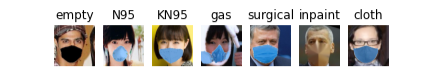
\includegraphics[scale=0.8]{images/mask_images.png}
	\caption{Synthetic Images generated by MaskTheFace}
\end{figure}

\subsection{Data Augmentation}
Data augmentation in data analysis are techniques used to increase the amount of data by adding slightly modified copies of already existing data or newly created synthetic data from existing data.
It acts as a regularizer and helps reduce overfitting when training a machine learning model. We calculated mean and std of train set, to apply normalization with transforms.Normalize().
\footnote[2] {We did not use normalization. train mean: [0.5033, 0.4229, 0.3915], train std: [0.2870, 0.2535, 0.2684]}

\begin{lstlisting}[language=Python]
    dataset_transform = torchvision.transforms.Compose([
            transforms.RandomHorizontalFlip(p=0.5),
            transforms.RandomVerticalFlip(p=0.5),
            transforms.RandomRotation((-135, 135)),
            transforms.RandomResizedCrop(size=(112,112),scale=(0.85, 1.0)),
            transforms.ToTensor(),
	    # transforms.Normalize(mean=TRAIN_MEAN, std=TRAIN_STD)
    ])
\end{lstlisting}

\subsection{Model Architecture}
The author of ResNet50 noted the Vanishing Gradient problem, which moves away from optimization as the model gets deeper.
By introducing Residual Block, which adds the input value as it is, the problem of forgetting the input was supplemented.
ResNet50 has a total of 50 layers, and each layer has a different form of residual block.
The figure below is a visual representation of the model structure.

\begin{figure}[H]
\centering

\includegraphics[scale=0.18]{images/resnet50_model.png}
\caption{Model Structure of ResNet50}

\end{figure}

\subsection{Model Training}
The hyperparameters applied when learning the model are as follows.
\begin{enumerate}[(1)]\setlength{\itemsep}{-1mm}
	\item input size: 3 $\times$ 112 $\times$ 112 (RGB image), output format: $\mathbb{R} \in (0, 1)$
	\item learning rate: 0.01
	\item the number of epochs: 50
	\item train data: 15,862, test data: 3,245
	\item batch size: 64
	\item optimizer: SGD with momentum = 0.9, weight decay = $5e^{-4}$
	\item loss function: torch.nn.BCEWithLogitsLoss
	\begin{equation} \label{crossentropy}
		l_n = -w_n[y_n \cdot \log \sigma (x_n) + (1 - y_n) \cdot \log (1 - \sigma (x_n))]
	\end{equation}

\item modification of model structure: ResNet50.fc = Linear(2048, 1)

\end{enumerate}

\section{Results}

\begin{figure}[H]
	\centering
	\subcaptionbox{Train Loss, Accuracy}[.22\textwidth] {
		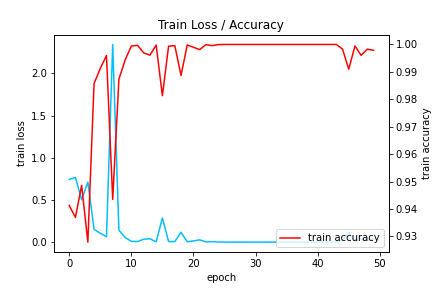
\includegraphics[scale=0.26]{images/train.png}
	}
	\subcaptionbox{Test Loss, Accuracy}[.22\textwidth] {
		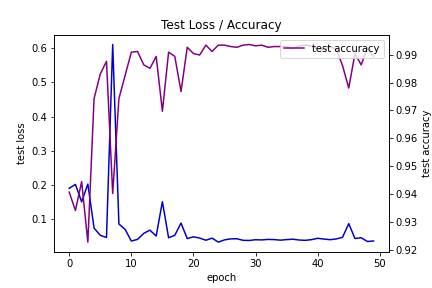
\includegraphics[scale=0.26]{images/test.png}
	}
	\subcaptionbox{Overall Loss, Accuracy}[.22\textwidth] {
		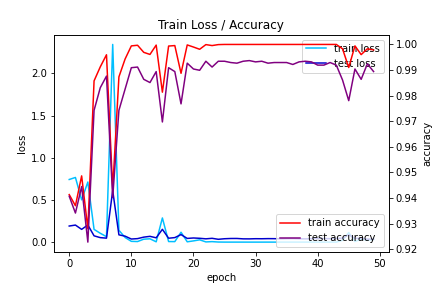
\includegraphics[scale=0.26]{images/train_test.png}
	}
	\subcaptionbox{Without Momentum}[.22\textwidth] {
		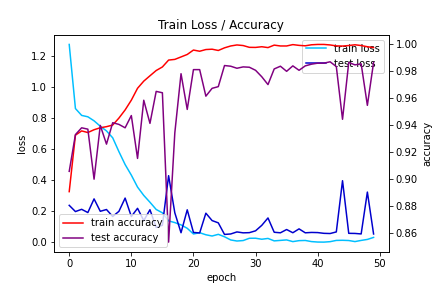
\includegraphics[scale=0.26]{images/train_test_without_momentum.png}
	}
	
	\caption{Model Train/Test Performance Plot. horizontal axis: epoch, vertical axis: accuracy(percentage), loss}
	\label{edafig}
\end{figure}

\begin{table}[h!]
	\centering
	
	\begin{tabular}{l|l|l|l}
		\toprule
		Metrics-1 & Loss & Metrics-2 & Accuracy(\%) \\
		\midrule
		Train Loss & 0.02047936655046101 & Train Accuracy & 99.82978186861682 \\
		Validation Loss & 0.03538672445137081 & Validation Accuracy & 99.24242424242424 \\
        
        \toprule
		Metrics-3 & Time Cost \\
		\midrule
        Elapsed Time in Training & 1 minute/epoch (approximation) \\
		\bottomrule
	\end{tabular}

	\vspace{0.2cm}
	\caption{Model Performance}
	\label{modelcomp}
\end{table}

\section{Conclusions}
In this project, transfer learning was conducted with ResNet50, and a model was constructed to detect whether a mask is worn in a given image.
Based on the test set, the accuracy was more than 99\%, and it was confirmed that the model properly classified most pictures even when the actual image was uploaded and tested.
\section{Discussions}

\subsection{Regularization technique - Early Stopping}
In machine learning, early stopping is a form of regularization used to avoid overfitting when training a learner with an iterative method, such as gradient descent.
\footnote[3] {https://en.wikipedia.org/wiki/Early\_stopping}

This technique was used to train our model. Compared to the test loss value in the previous epoch for each iteration, the model parameter was stored only when the test value was smaller than before.
Therefore, if the overfitting occurs and the test loss is larger than before, the result is not reflected, indirectly applying early stopping technique.

\subsection{Momentum}
Gradient descent can oscillate when it enters a narrow valley with large learning rate.
We can enforce a bit smoother trajectory by adding an additional term to gradient descent called "momentum".
It prevents oscillative movement in a valley.
The presence of momentum in the learning process had a great influence on the degree of improvement in the local minima.
It can be seen from Figures 3-(c) and (d) that there is a large difference in terms of loss and accuracy.

\subsection{Limitations of the current model}
The ResNet50 determines the image based on the texture shown in the image.
The characteristics of the model become a limitation when measuring whether or not a mask is actually worn.
This experiment was done with the pretrained ResNet-50 architecture to examine its limitations.
Both of the pictures below are non-masked.
The image covered with hands was judged to be non-masked because the textures of the face and hands were similar, but when the face was covered with a notebook rather than a hand, it was judged to be masked because the textures were clearly different.
In addition, when the model was trained without any pretrained parameters, the model only detected the correct mask types which is in the MaskTheFace dataset.
To compensate for these drawbacks, it is necessary to establish a model capable of separately recognizing objects for masks in future studies.


\section{Qualitative Evaluation}
In order to flexibly determine the performance of the model, the author's mask-wearing photo and mask-free photo were arbitrarily converted to 112 $\times$ 112 size and entered.
The trained model returns one real number between 0 and 1 for each image, since the last layer consists of a sigmoid.
With 0.5 as the boundary value, the closer to 0, the less the mask was worn, and the closer to 1, the more the mask was worn.
The model returned a value of 0.02862 for the first picture(non-masked) and 1.0 for the second picture(masked).
Thus, the trained model properly classifies whether or not to wear a mask in the input picture.

\begin{figure}[H]
\centering
\subcaptionbox{Limitations of ResNet50-based Model}[.4\textwidth] {
	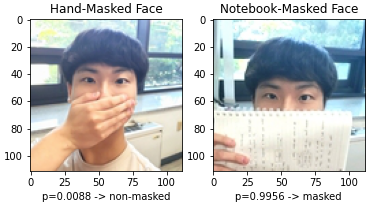
\includegraphics[scale=0.4]{images/result2.png}
}
\subcaptionbox{Model Qualification with real images}[.4\textwidth] {
	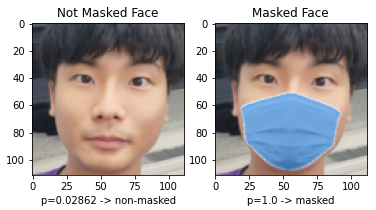
\includegraphics[scale=0.4]{images/result.png}
}

\end{figure}

\end{document}